\documentclass[12pt,a4paper]{scrartcl}
\usepackage{graphicx} % Required for inserting images
\usepackage{verbatim}
\usepackage{listings}
\usepackage{wrapfig}
\usepackage{times}
\usepackage{float}
\usepackage[a4paper, left=2cm, right=2cm, top=2cm, bottom=3.5cm]{geometry}
\usepackage[dvipsnames]{xcolor}
\usepackage{hyperref}
\usepackage{tocloft}
\setlength{\cftbeforetoctitleskip}{-4em}
% Links on toc
\hypersetup{
    colorlinks,
    citecolor=black,
    filecolor=black,
    linkcolor=black,
    urlcolor=black
}


\title{Relazione Prova finale di Reti Logiche}
\author{
    \textbf{Francesco Caracciolo} \\
    \small{Codice Persona: \texttt{10796701}} \small{Matricola: \texttt{980989}}
}
\date{}
\lstset{
  basicstyle=\ttfamily,
  keywordstyle=\color{blue}\bfseries,
  commentstyle=\color{green},
  stringstyle=\color{red},
  numbers=left,
  numberstyle=\tiny,
  backgroundcolor=\color{white},
  tabsize=2,
  frame=single,
  showtabs=false,
  showspaces=false,
  breaklines=true,
  breakatwhitespace=true,
  captionpos=b,
  float=tbp,
}

\begin{document}
\maketitle
\tableofcontents
\newpage
\section{Introduzione}
\subsection{Obiettivo del progetto}
Il progetto consiste nello sviluppare un componente hardware nel linguaggio VHDL che ha il compito di scansionare una sequenza di misurazioni presenti in memoria ed associare ad ogni misurazione un relativo valore di confidenza. \newline
Le misurazioni con valore 0 hanno il significato di "valore non specificato", fanno quindi calare la confidenza della misurazione.
\subsection{Specifica del funzionamento}
Ogni misurazione W può assumere un valore compreso tra 0 e 255 (quindi ha dimensione di 8 bit, ovvero 1 byte, in memoria).
\newline Nell'indirizzo di memoria successivo a ogni misurazione è presente un byte che il componente deve completare con il valore di confidenza C.
\begin{itemize}
    \item Ogni volta che si incontra una misurazione diversa da 0, la confidenza viene impostata a 31.
    \item Ogni volta che si incontra una misurazione uguale a 0, la confidenza, se maggiore di 0, viene decrementata.
\end{itemize}
Inoltre, il componente deve rimpiazzare le misurazioni non specificate con l'ultima misurazione valida. Se la sequenza inizia con valori non specificati (0), allora la confidenza parte da 0 e considera 0 tutti i valori.\newline
In seguito un esempio:
\newline Sequenza Iniziale: \newline
[\textcolor{ForestGreen}{177}, \textcolor{gray}{0}, \textcolor{ForestGreen}{109}, \textcolor{gray}{0}, \textcolor{ForestGreen}{249}, \textcolor{gray}{0}, \textcolor{red}{0}, \textcolor{gray}{0}, \textcolor{red}{0}, \textcolor{gray}{0}, \textcolor{red}{0}, \textcolor{gray}{0}, \textcolor{ForestGreen}{102}, \textcolor{gray}{0}, \textcolor{red}{0}, \textcolor{gray}{0}]
\newline Sequenza finale: \newline
[\textcolor{ForestGreen}{177}, 31, \textcolor{ForestGreen}{109}, 31, \textcolor{ForestGreen}{249}, 31, \textcolor{red}{249}, 30, \textcolor{red}{249}, 29, \textcolor{red}{249}, 28, \textcolor{ForestGreen}{102}, 31, \textcolor{red}{102}, 30]

\newpage
\subsection{Specifica hardware}
\begin{figure}[htbp]
  \centering
  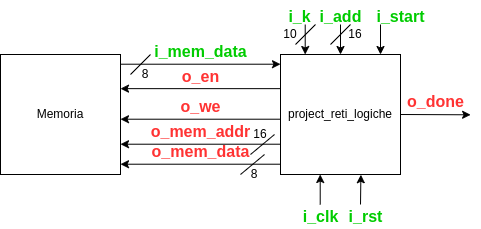
\includegraphics[width=0.8\linewidth]{base_component.drawio.png}
  \caption{Rappresentazione schematica degli ingressi e delle uscite del componente.}
  \label{fig:componente}
\end{figure}

\paragraph{Ingressi} 
    \begin{itemize}
        \item i\_clk: segnale di clock;
        \item i\_rst: segnale di reset;
        \item i\_add: vettore da 16 bit, indirizzo di memoria a partire da cui inizia la sequenza;
        \item i\_k: vettore da 10 bit, numero di misurazioni da elaborare nella sequenza;
        \item i\_start: segnale di inizio della computazione; 
        \item i\_mem\_data: vettore da 8 bit, contenuto della memoria all'indirizzo richiesto in precedenza; 
    \end{itemize}
\paragraph{Uscite} 
    \begin{itemize}
        \item o\_done: alto quando l'elaborazione è stata completata e non è stato ancora dato il segnale di start;
        \item o\_en: abilita la memoria;
        \item o\_we: abilita la scrittura in memoria;
        \item o\_mem\_addr: vettore da 16 bit, indica l'indirizzo di memoria su cui scrivere/leggere;
        \item o\_mem\_data: vettore da 8 bit, indica il valore da scrivere in memoria se o\_en è abilitato;
    \end{itemize}
Al componente verrà sempre dato un segnale di reset prima della prima elaborazione, inoltre deve essere in grado di gestire più elaborazioni senza un segnale di reset intermedio.
\newpage
\section{Architettura}
\begin{figure}[htbp]
  \centering
  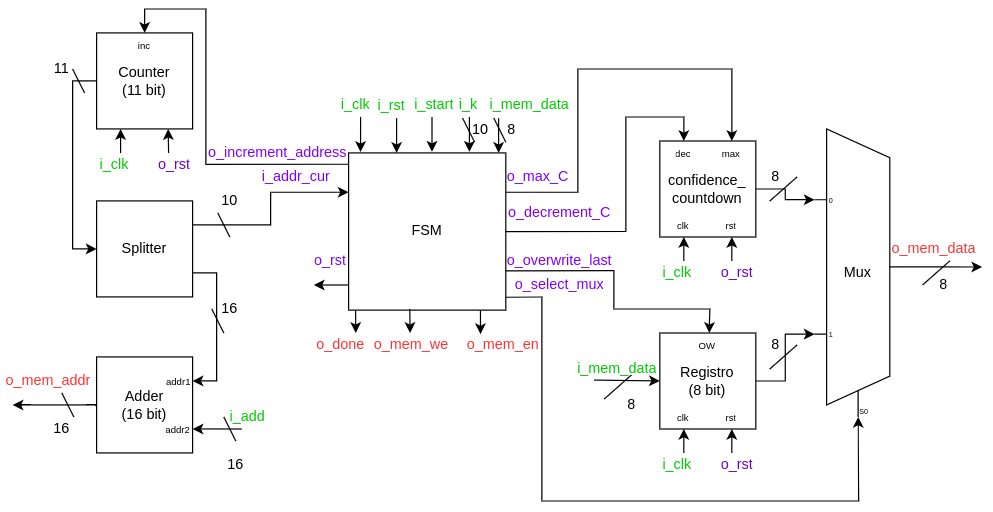
\includegraphics[width=1\linewidth]{schema.drawio2.png}
  \caption{ Struttura della rete
        \newline
        In \textcolor{red}{rosso} sono rappresentate le \textcolor{red}{uscite principali} del componente. \newline
        In \textcolor{green}{verde} sono rappresentate le \textcolor{green}{entrate principali} del componenete. \newline
        In \textcolor{violet}{viola} sono rappresentati i \textcolor{violet}{segnali} della macchina a stati.
    }
  \label{fig:componente}
\end{figure}
    Il sistema è composto da 7 componenti, in seguito analizzati approfonditamente:
    \begin{itemize}
        \item \textbf{FSM}: Macchina a stati finiti che si occupa di gestire i segnali degli altri componenti e della gestione dello stato;
        \item \textbf{confidence\_countdown}: Un semplice decrementatore che serve per la gestione della confidenza. Ha un ingresso \textit{MAX} che
                imposta il valore contenuto a 31, mentre \textit{DEC} decrementa il valore fino allo 0;
        \item \textbf{reg\_8}: un registro a 8 bit che serve a mantenere l'ultima misurazione valida;
        \item \textbf{multiplexer}: sceglie cosa scrivere in memoria, con \textit{sel} a 0 scrive la confidenza, con \textit{sel} a 1 scrive l'ultima misurazione utile;
        \item \textbf{counter}: un contatore a 11 bit che fa da cursore per l'indirizzo di memoria su cui si sta operando attualmente;
        \item \textbf{splitter}: questo componente divide il segnale risultante dal counter in due segnali:
            \begin{itemize}
                \item un segnale a 16 bit che è semplicemente l'output del counter esteso;
                \item un segnale a 10 bit che è utilizzato dalla macchina a stati e indica quante misurazioni sono state lette (cursore/2); 
            \end{itemize}
        \item \textbf{adder}: un semplice adder senza carry, ha il ruolo di calcolare l'indirizzo di memoria su cui si sta operando sommando al 
                    valore \textcolor{green}{i\_add}, il valore del cursore;
    \end{itemize}

    \subsection{Confidence Countdown}
    \begin{figure}[htbp]
      \centering
      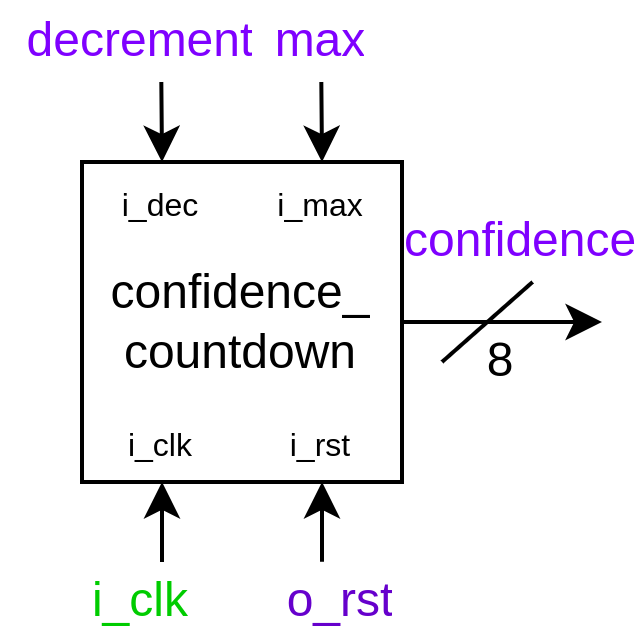
\includegraphics[width=0.6\linewidth]{schema-confidence_countdown.png}
      \caption{Rappresentazione schematica degli ingressi e delle uscite del componente.}
      \label{fig:componente}
    \end{figure}
    Confidence Countdown è un componente sincrono che ha lo scopo di salvare il valore della confidenza durante l'esecuzione, portarlo al valore massimo (31) in un ciclo di clock quando necessario, e decrementarlo.
    \subsubsection{Interfaccia}
    \begin{itemize}
        \item i\_clk: segnale di clock;
        \item i\_rst: segnale di reset, porta il valore contenuto nel componente a 0; 
        \item i\_dec: decrementa il valore contenuto nel componente;
        \item i\_max: imposta il valore contenuto nel componente a 31;
        \item o\_C: uscita del componente a 8 bit;
    \end{itemize}
    Il segnale di reset porta il contenuto 0 dato che all'inizio dell'esecuzione, se non viene letta alcuna misurazione valida, la confidenza è nulla. 
    \newpage
    \subsubsection{Architettura}
    \begin{lstlisting}[language=VHDL]
architecture confindence_countdown_arch of confidence_countdown is
signal stored_value : std_logic_vector(4 downto 0) := "00000";
begin
  o_C <= "000" & stored_value;
  process (i_clk, i_rst, i_max)
  begin
      if i_rst = '1' then
          stored_value <= (others => '0');
      elsif rising_edge(i_clk) then
        if i_max = '1' then
            stored_value <= (others => '1');
        elsif i_dec = '1' then
            if stored_value /= "00000" then
                stored_value <= stored_value - 1;
            end if;
        end if;
      end if;
    end process;
end confindence_countdown_arch;
    \end{lstlisting}
    L'architettura del componente è costituita da un processo in cui il segnale di reset è asincrono, mentre gli altri segnali sono sincroni con il clock. \newline
    Il segnale \textit{stored\_value} è a 5 bit dato che questo componente deve elaborare solo valori tra 0 e 31, viene poi esteso a 8 bit in modo da essere scritto in memoria (8 bit) più agevolmente. \newline
    Quando il segnale \textit{i\_max} è alto, il valore viene portato a 31, mentre quando \textit{i\_max} è basso e \textit{i\_dec} è alto, il valore viene decrementato di uno. \newline Il valore salvato viene sempre dato in output.
    \newpage
    \subsection{Registro a 8 bit}
        \begin{figure}[htbp]
          \centering
          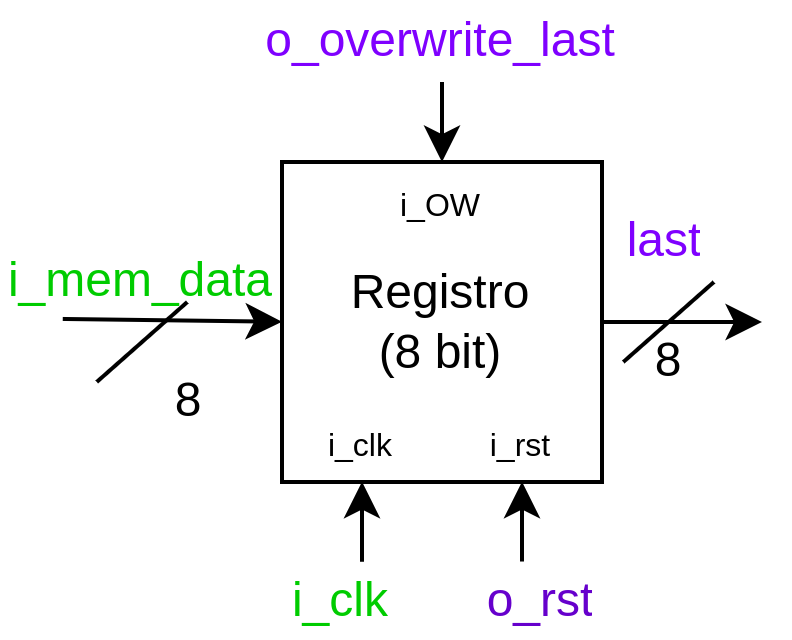
\includegraphics[width=0.6\linewidth]{schema-reg_8.drawio.png}
          \caption{Rappresentazione schematica degli ingressi e delle uscite del componente.}
          \label{fig:componente}
        \end{figure}
    Questo componente (reg\_8) è un semplice registro sincrono a 8 bit che ha il ruolo di salvare l'ultima misurazione valida.
    \subsubsection{Interfaccia}
    \begin{itemize}
        \item i\_clk: segnale di clock;
        \item i\_rst: segnale di reset, asincrono, porta il valore contenuto nel registro a 0;
        \item i\_overwrite: se alto sovrascrive il valore contenuto nel registro con il valore di \textit{i\_value};
        \item i\_value: valore a 8 bit da inserire nel registro se \textit{i\_overwrite} è alto;
        \item output: uscita del registro a 8 bit con l'ultimo valore salvato;
    \end{itemize}
    Dato che in questo componente vengono salvati solo dati in memoria, \textit{i\_value} è direttamente collegato all'entrata principale \textit{i\_mem\_data}.
    L'architettura di questo componente è omessa perché banale.
    \newpage
    \subsection{Multiplexer}
        \begin{figure}[htbp]
          \centering
          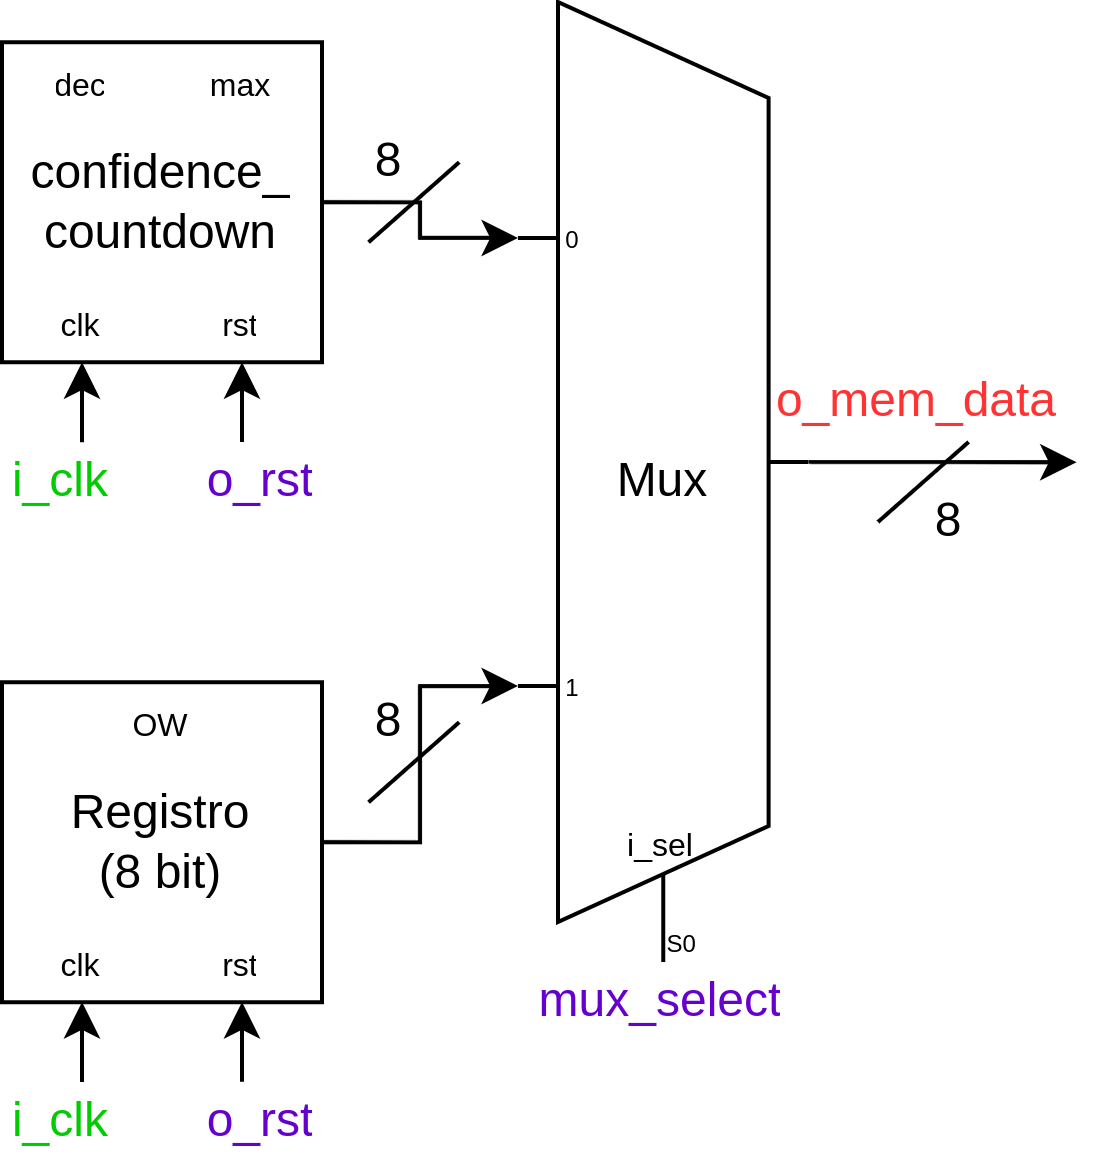
\includegraphics[width=0.4\linewidth]{schema-mux.drawio.png}
          \caption{Rappresentazione schematica degli ingressi e delle uscite del componente nel contesto in cui si trova.}
          \label{fig:componente}
        \end{figure}
     Questo componente è un semplice multiplexer da due ingressi a 8 bit. Il suo ruolo è quello di gestire cosa viene scritto in memoria.
     Se \textit{sel} è 0 viene scritta la confidenza (da \textit{confidence\_countdown}), mentre se \textit{sel} è 1 viene scritta l'ultima misurazione valida contenuta in \textit{reg\_8}.
    \subsection{Counter}
        \begin{figure}[htbp]
            \centering
            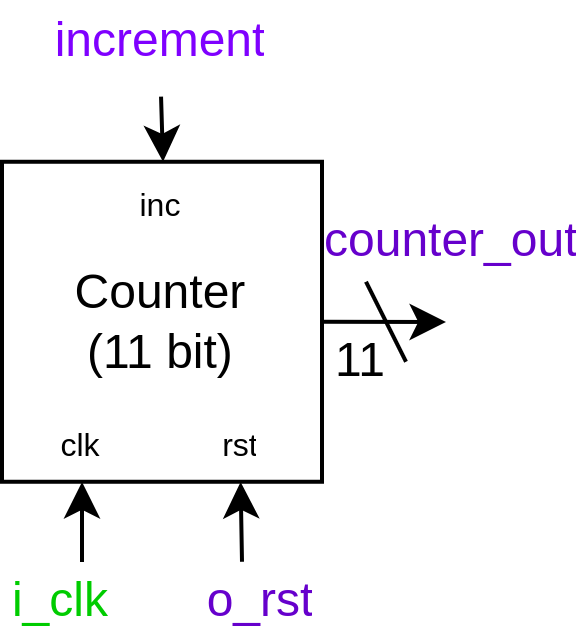
\includegraphics[width=0.4\linewidth]{schema-Counter.drawio.png}
            \caption{Rappresentazione schematica degli ingressi e delle uscite del componente.}
            \label{fig:componente}
        \end{figure}
    Questo componente è un semplice contatore sincrono a 11 bit che ha il compito di conteggiare quanti indirizzi di memoria sono stati elaborati e di fungere da cursore per l'indirizzo di memoria su cui si sta operando.
    \newline L'output del contatore viene sfruttato in due modi:
    \begin{itemize}
        \item Viene aggiunto all'ingresso \textcolor{green}{i\_add} per stabilire su quale indirizzo si stia operando e costituire l'uscita \textcolor{red}{o\_mem\_addr}.
        \item I 10 bit più significativi (l'output numerico del contatore è quindi diviso per due) sono sfruttati dalla macchina a stati finiti per stabilire quante misurazioni sono state elaborate ed eventualmente terminare la computazione.
     \end{itemize}
     \subsubsection{Interfaccia}
            \begin{itemize}
                \item i\_clk: segnale di clock;
                \item i\_rst: segnale di reset, porta il valore del contatore a 0;
                \item i\_increment: se alto incrementa di 1 il valore del contatore per ogni ciclo di clock;
                \item output: uscita del contatore;
            \end{itemize}
        \subsubsection{Architettura}
            \begin{lstlisting}[language=VHDL]
architecture counter_arch of counter is
signal stored_value: std_logic_vector(10 downto 0) := "00000000000";
begin
    output <= stored_value;
    process (i_clk, i_rst)
    begin
    if i_rst = '1' then
        stored_value <= (others => '0');
    elsif rising_edge(i_clk) then
        if increment = '1' then
            stored_value <= stored_value + 1;
        end if;
    end if;
    end process;
end counter_arch;
            \end{lstlisting}
            L'architettura del componente è costituita da un processo in cui il segnale di reset è asincrono, mentre gli altri segnali sono sincroni con il clock.
            \newline Il segnale \textit{stored\_value} è un vettore da 11 bit.
            \newline In uscita viene sempre dato il valore di \textit{stored\_value}.
            \newline Quando il reset è 1, indipendentemente dal clock, il contenuto di \textit{stored\_value} viene impostato a 0, dato che al reset del componente, non è stato ancora letto alcun indirizzo di memoria.
            \newline Sul fronte di salita del clock, se \textit{increment} è alto, il valore contenuto all'interno di \textit{stored\_value} viene incrementato, altrimenti rimane invariato.
    \subsection{Splitter}
        \begin{figure}[H]
            \centering
            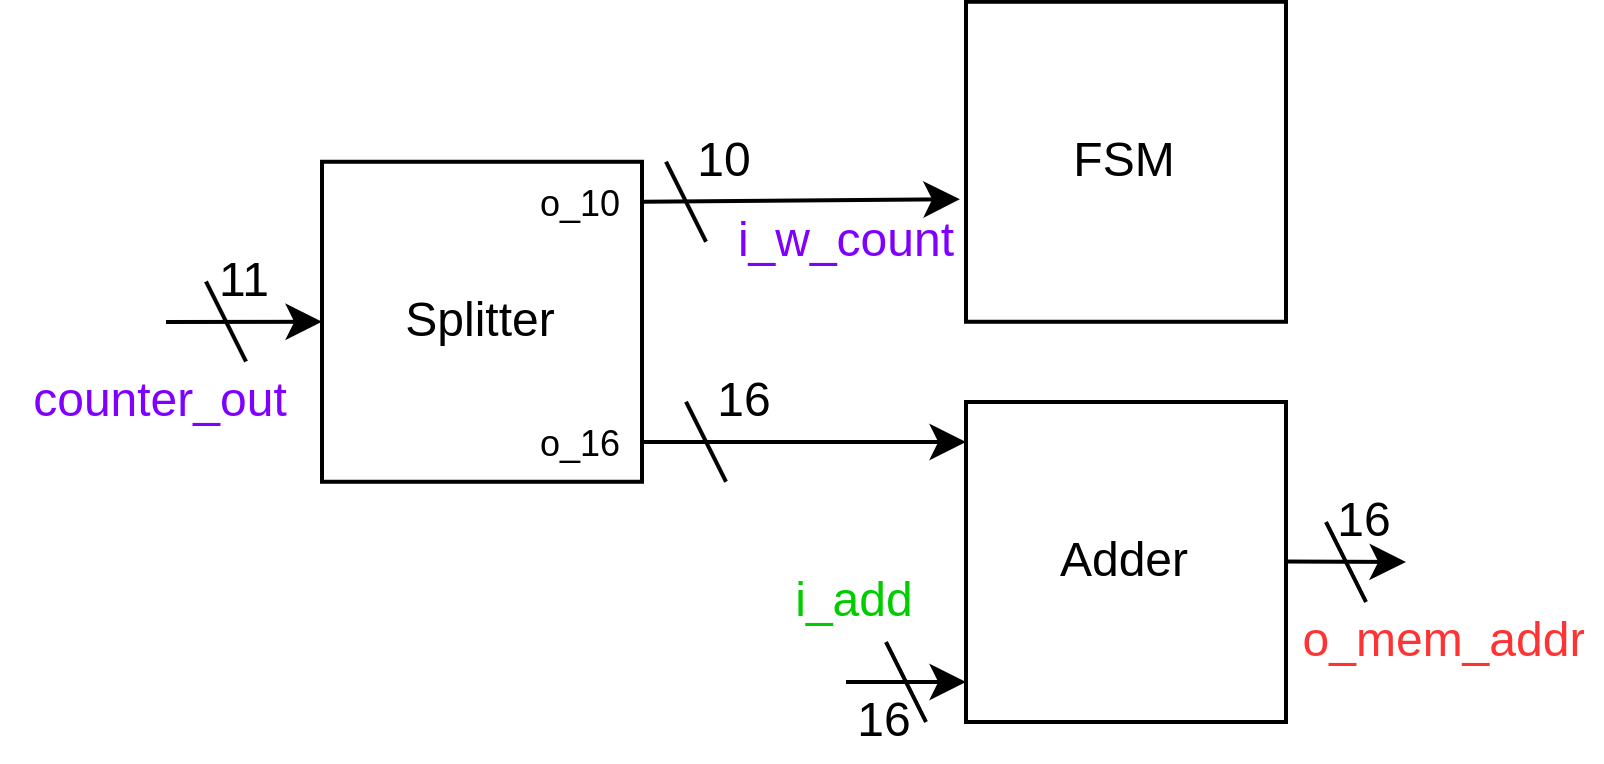
\includegraphics[width=\linewidth]{schema-splitter.drawio.png}
            \caption{Rappresentazione schematica degli ingressi e delle uscite del componente nel contesto in cui si trova (FSM semplificata)}
            \label{fig:componente}
        \end{figure}
    Lo splitter è un componente asincrono che da un segnale in input a 11 bit, lo divide in due segnali in output:
    \begin{itemize}
        \item Un segnale a 10 bit composto dai primi 10 bit del vettore in ingresso. Ha l'utilità pratica di dividere il valore in ingresso per due (arrotondato per difetto). \newline All'interno della rete logica ha il compito di "informare" la macchina a stati finiti di quante misurazioni sono state lette in memoria.
        \item Un segnale a 16 bit che è l'estensione del segnale a 11 bit in ingresso, in modo da essere compatibile con l'adder.
    \end{itemize}
    \textbf{Nota:} questo componente non è strettamente necessario per la rete, un modo alternativo per ottenere lo stesso risultato è quello di collegare nel port mapping solo una parte del vettore di bit \textcolor{violet}{counter\_out} alla macchina a stati ed estendere il valore in entrata per l'adder.
    \newline Ho optato per questa soluzione poiché la ritenevo più chiara all'interno della rappresentazione e più modulare in caso di modifiche all'architettura.
    \subsubsection{Interfaccia}
        \begin{itemize}
            \item input: segnale a 11 bit in input;
            \item o\_10: segnale a 10 bit in output contenente i 10 bit più significativi del segnale d'ingresso;
            \item o\_16: segnale a 16 bit in output che è un'estensione del valore d'ingresso a 16 bit; 
        \end{itemize}
    \subsubsection{Architettura}
        \begin{lstlisting}[language=VHDL]
architecture splitter_arch of splitter is

begin
    o_10 <= input(10 downto 1);
    o_16 <= "00000" & input;
end splitter_arch;
        \end{lstlisting}
        L'uscita o\_10 è data dai primi 10 bit dell'input.
        \newline L'uscita o\_16 è ottenuta concatenando l'input ad un vettore di bit contenente quattro zeri.
    \subsection{Adder}
        \begin{figure}[htbp]
            \centering
            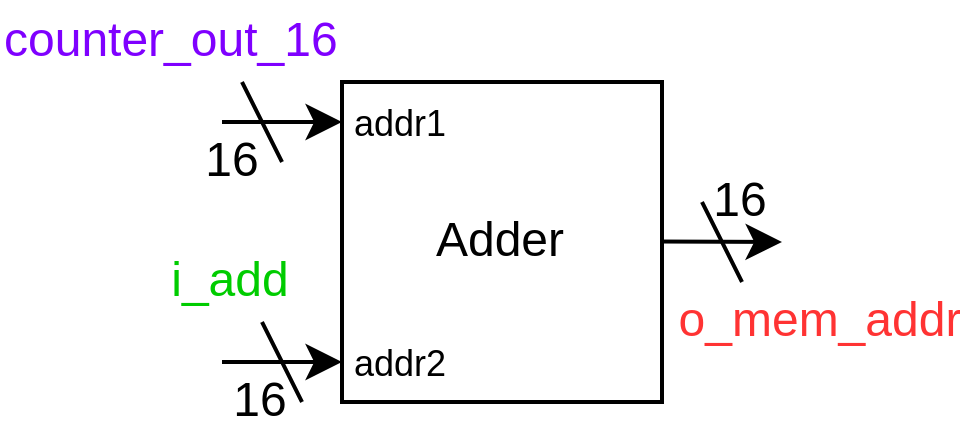
\includegraphics[width=0.8\linewidth]{schema-adder.drawio.png}
            \caption{Rappresentazione schematica degli ingressi e delle uscite del componente.}
            \label{fig:componente}
        \end{figure}
        Questo componente ha il compito di sommare due numeri a 16 bit senza segno e senza carry. Nella rete logica, l'adder ha il ruolo di sommare all'indirizzo di memoria da cui inizia la sequenza ( segnale \textcolor{green}{i\_add}), il cursore di memoria, ovvero l'output esteso del counter, restituendo quindi l'indirizzo su cui operare (\textcolor{red}{o\_mem\_addr}).  
        \newline Il carry non serve in questo caso dato che nessun indirizzo di memoria è espresso con più di 16 bit. Nel caso in cui venga data una combinazione di segnali tali che \(i\_add + i\_k*2\) sia maggiore del massimo indirizzo di memoria, si sta violando la specifica e il comportamento del componente \textit{project\_reti\_logiche} non è specificato.
    \subsubsection{Interfaccia}
            \begin{itemize}
                \item addr1: ingresso, vettore da 16 bit
                \item addr2: ingresso, vettore da 16 bit
                \item out: uscita, somma a 16 bit senza segno di \textit{addr1} e \textit{addr2} senza carry
            \end{itemize}
    \newpage
    \subsection{Macchina a stati}
        \begin{figure}[htbp]
          \centering
          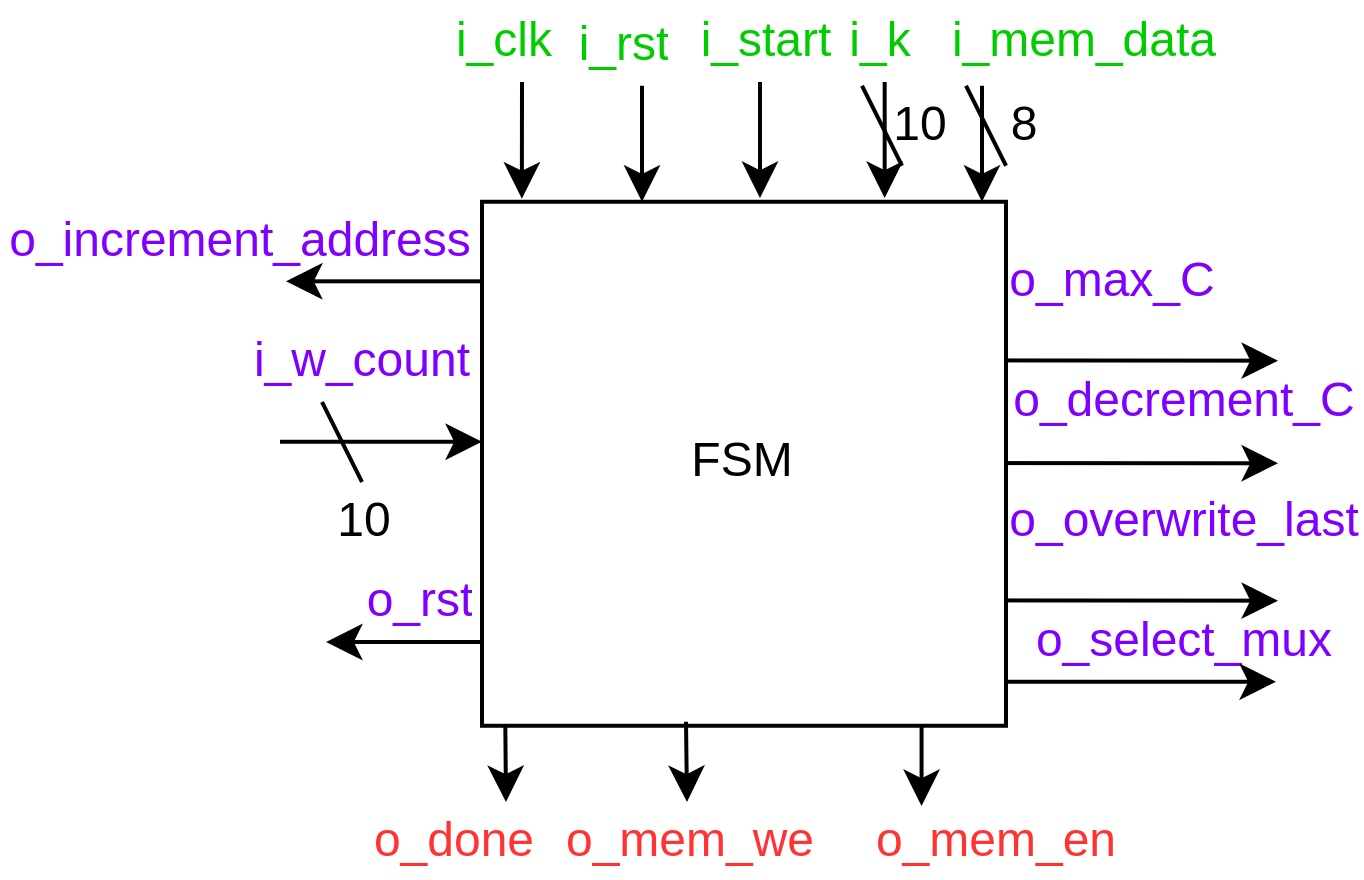
\includegraphics[width=0.9\linewidth]{schema-fsm.drawio.png}
          \caption{Rappresentazione schematica degli ingressi e delle uscite della macchina a stati.
          \newline In \textcolor{green}{verde} sono rappresentate le entrate principali
          \newline In \textcolor{red}{rosso} sono rappresentate le uscite principali
          \newline In \textcolor{violet} viola sono rappresentati i segnali interni al componente}
          \label{fig:componente}
        \end{figure}
        La macchina a stati ha il compito di gestire in comportamento sequenziale del componente e di tutti i moduli di cui è composto. 
        \newline La rete è stata progettata in modo che l'FSM si occupi solo di alzare/abbassare segnali e di fare confronti.
        \newpage
        \subsubsection{Interfaccia}
            \begin{itemize}
                \item \textcolor{green}{i\_clk, i\_rst, i\_start, i\_k, i\_mem\_data} sono gli ingressi principali del componente \textit{project\_reti\_logiche}
                \item \textcolor{red}{o\_done, o\_mem\_we, o\_mem\_en} sono le uscite principali del compontente \textit{project\_reti\_logiche}
                \item \textbf{i\_w\_count} è un vettore da 10 bit in ingresso fornito dal contatore che indica quante parole sono state elaborate fino a quel momento. Serve ad essere confrontato con \textit{i\_k} per stabilire quando l'esecuzione è terminata.
                \item \textbf{o\_rst} è un segnale interno che viene dato ai componenti che necessitano di reset. La motivazione per cui i moduli non usano il segnale \textit{i\_rst} principale è perché a fine esecuzione è necessario mandare un segnale di reset ai vari componenti per permetterne il corretto funzionamento in caso di una seconda esecuzione senza un segnale di reset esterno.
                \item \textbf{o\_max\_C} è un segnale che viene dato al compontente \textit{confidence\_countdown} per impostare il massimo valore di confidenza (33)
                \item \textbf{o\_decrement\_C} è un segnale che viene dato al componente \textit{confidence\_countdown} per decrementare il valore di confidenza
                \item \textbf{o\_overwrite\_last} è un segnale che viene dato al registro a 8 bit per indicare di sovrascrivere l'ultima misurazione valida salvata nel registro
                \item \textbf{o\_select\_mux} sceglie cosa scrivere in memoria (quando \textit{o\_mem\_we} e \textit{o\_mem\_en} sono alti). Vale 0 per scrivere la confidenza, vale 1 per scrivere l'ultima misurazione valida contenuta nel registro.
                \item \textbf{o\_increment\_address} è un segnale dato al counter per incrementare il cursore dell'indirizzo di memoria
            \end{itemize}
        \subsubsection{Architettura}
            La macchina a stati è composta da 9 stati e implementata tramite due processi:
            \begin{itemize}
                \item Un processo che gestisce le transizioni di stato
                \item Un processo che gestisce i segnali in funzione dello stato in cui si trova
            \end{itemize}
            \begin{figure}[htbp]
              \centering
              \includegraphics[width=1\linewidth]{fsm.png}
              \caption{Diagramma delle transizioni della macchina a stati}
              \label{fig:componente}
            \end{figure}
            \newpage
            \paragraph{Transizioni degli stati} Le transizioni di stato sono sincrone con il clock. In seguito un estratto del codice dell'architettura:
            \begin{lstlisting}[language=VHDL]
architecture fsm_arch of fsm is
    type S is (IDLE, CHECK_ADDR, DONE,READ_MEM_DATA, 
                    SAVE_VALUE, CUR_INC, MEM_WRITE,
                    MEM_WRITE_0, CUR_INC_0, WRITE_C);
    signal curr_state : S := IDLE;
begin
    -- State transitions
    process(i_clk, i_rst)
    begin
        if i_rst = '1' then
            curr_state <= IDLE;
        elsif rising_edge(i_clk) then
            case curr_state is
                when IDLE => 
                    if i_start = '1' then
                        curr_state <= CHECK_ADDR;
                    else
                        curr_state <= IDLE;
                    end if;
        [...]
            \end{lstlisting}
            Definisce un tipo enumerato \textit{S} per rappresentare i possibili stati della macchina a stati e un segnale \textit{curr\_state} per salvare lo stato attualmente in esecuzione.
            \newline In modo asincrono, il reset imposta lo stato iniziale "IDLE".
            \newline Sul fronte di salita del ciclo di clock, invece, avvengono le transizioni di stato in base allo stato attuale e ad eventuali condizioni aggiuntive.
            \newline Il diagramma sovrastante indica tutte le altre transizioni di stato.
            \paragraph{Gestione dei segnali} I segnali sono gestiti da un altro processo che si occupa solo di alzare o abbassare segnali in funzione dello stato corrente.
            \newline Per evitare latch, tutti i segnali hanno come valore predefinito 0 all'inizio del processo.
            \begin{lstlisting}[language=VHDL]
    process(curr_state)
    begin
        o_mem_we <= '0';
        o_mem_en <= '0';
        o_done <= '0';
        o_max_C <= '0';
        o_decrement_C <= '0';
        o_select_mux <= '0';
        o_overwrite_last <= '0';
        o_increment_address <= '0';
        o_rst <= '0';
            \end{lstlisting}
            \textbf{Nota:} all'interno del codice riguardante i singoli stati, ho ripetuto l'istruzione che causa lo spegnimento di alcuni segnali per una maggiore leggibilità e sequenzialità di lettura, anche se a livello di codice non hanno alcun effetto. 
            \newline \newline Analizziamo cosa avviene nei singoli stati.
            \subparagraph{IDLE} Idle ha il solo scopo di aspettare che il segnale \textit{i\_start} diventi 1 per poter proseguire con l'elaborazione. Mentre è in \textit{IDLE}, la FSM dà il segnale di reset agli altri moduli in modo da permettere la corretta inizializzazione in caso di esecuzioni multiple senza che sia dato il segnale \textit{i\_rst} tra di esse.
                \begin{lstlisting}[language=VHDL]
        case curr_state is
            when IDLE =>
                o_rst <= '1';
                \end{lstlisting}
            \subparagraph{CHECK\_ADDR} Questo stato ha lo scopo di controllare se la quantità di misurazioni elaborate (\textit{i\_w\_count}) è uguale al valore \textit{i\_k} in modo da stabilire se la computazione deve terminare. Se i due valori sono uguali, l'esecuzione è terminata e passa allo stato \textit{DONE}, altrimenti l'esecuzione avanza allo stato \textit{READ\_MEM\_DATA}.
                \newline Viene raggiunto ogni volta che la computazione di una misurazione è terminata.
                \begin{lstlisting}[language=VHDL]
            when CHECK_ADDR =>
                -- Setup memory
                o_mem_we <= '0';
                o_mem_en <= '1';
                -- Fix increments
                o_max_C <= '0';
                -- Stop ad_cur
                o_increment_address <= '0';
                \end{lstlisting}
                Lo stato alza il segnale \textit{o\_mem\_en} in modo da richiedere la lettura del valore in memoria nello stato successivo \textit{READ\_MEM\_DATA}. I segnali abbassati servono ad indicare che le azioni di stati precedenti sono interrotte.
            \subparagraph{READ\_MEM\_DATA}
                Questo stato ha il solo scopo di leggere la misurazione in memoria e stabilire se è maggiore di 0. Nel caso in cui sia 0 passa allo stato \textit{MEM\_WRITE\_0}, altrimenti passa allo stato \textit{SAVE\_VALUE}.
            \subparagraph{SAVE\_VALUE}
                Questo stato viene raggiunto nel caso in cui si stia analizzando una misurazione maggiore di 0, quindi valida.
                \begin{lstlisting}[language=VHDL]
            when SAVE_VALUE =>
                -- Maximize confidence
                o_max_C <= '1';
                -- Save W in reg_8
                o_overwrite_last <= '1';
                o_mem_en <= '1';
                 \end{lstlisting}
                 In questo stato vengono effettutate due azioni:
                    \begin{enumerate}
                        \item Viene massimizzata la confidenza con il segnale \textit{o\_max\_C}
                        \item Viene salvata la misurazione nel registro in modo da poterla utilizzare come ultima misurazione valida nel caso in cui venga incontrato uno 0. Per salvare la misurazione abilito il segnale di overwrite e la memoria per permettere la lettura del valore.
                    \end{enumerate}
                \subparagraph{CUR\_INC} Questo stato ha il ruolo di incrementare la posizione del cursore in memoria di uno per raggiungere l'indirizzo su cui successivamente andrà scritto il valore di confidenza.
                \begin{lstlisting}[language=VHDL]
            when CUR_INC =>
                -- Stop confidence maximizing
                o_max_C <= '0';
                -- Stop W saving
                o_overwrite_last <= '0';
                -- Increase memory cursor
                o_increment_address <= '1';
                 \end{lstlisting}
                 \textit{o\_increment\_address} è il segnale che incrementa il counter che si occupa di fare da cursore per la memoria.
                 \newline I segnali di \textit{max} e \textit{overwrite} vengono abbassati dato che non è più necessario massimizzare la confidenza o sovrascrivere il valore nel registro con il valore in memoria.

                \subparagraph{MEM\_WRITE\_0} Questo è il primo stato dell'elaborazione nel caso in cui \textit{i\_mem\_data} = 0.
                    \newline Lo scopo di questo stato è quello di scrivere l'ultima misurazione valida in memoria e decrementare la confidenza.
                 \begin{lstlisting}[language=VHDL]
            when MEM_WRITE_0 =>
                -- Write value of register (last W) in memory
                o_select_mux <= '1';
                o_mem_we <= '1';
                o_mem_en <= '1';
                -- Decrease Confidence
                o_decrement_C <= '1';
                 \end{lstlisting} 
                 \textit{o\_select\_mux} a 1 seleziona il valore del registro come valore da scrivere in memoria. I segnali \textit{o\_mem\_we} e \textit{o\_mem\_en} sono necessari per permette che il valore venga scritto in memoria.
                 \newline Il segnale \textit{o\_decrement\_C} alto decrementa il valore di confidenza contenuto nel modulo \textit{confidence\_countdown} di 1.

                 \subparagraph{CUR\_INC\_0} Questo è il secondo stato dell'elaborazione nel caso in cui \textit{i\_mem\_data} = 0.
                    \newline Lo scopo di questo stato è quello di incrementare il cursore dell'indirizzo di memoria in modo da scrivere nello stato successivo la confidenza in memoria.
                 \begin{lstlisting}[language=VHDL]
            when CUR_INC_0 =>
                -- Stop writing
                o_mem_we <= '0';
                o_mem_en <= '0';
                -- Increase address cursor
                o_increment_address <= '1';
                -- Stop confidence decrement
                o_decrement_C <= '0';
                 \end{lstlisting} 
                 I segnali \textit{o\_mem\_we} e \textit{o\_mem\_en} vengono abbassati dato che non ci sono operazioni da fare in memoria.
                 \newline Il segnale \textit{o\_decrement\_C} viene abbassato dato che non è più necessario decrementare la confidenza.
                 \newline \textit{o\_increment\_address} viene alzato per aumentare il cursore di memoria e scrivere la confidenza nello stato successivo.
                 
                 \subparagraph{WRITE\_C} Questo è il terzo e ultimo stato dell'elaborazione della singola misurazione.
                    \newline Lo scopo di questo stato è quello di scrivere il valore della confidenza in memoria ed incrementare il cursore di memoria.
                 \begin{lstlisting}[language=VHDL]
            when WRITE_C =>
                -- Write confidence
                o_select_mux <= '0';
                o_mem_we <= '1';
                o_mem_en <= '1';
                -- Increase address
                o_increment_address <= '1';
                 \end{lstlisting} 
                 Il segnale \textit{o\_select\_mux} è 0 per indicare che in memoria va scritta la confidenza. I segnali \textit{o\_mem\_we} e \textit{o\_mem\_en} sono necessari per permettere che il valore venga scritto in memoria.
                 \newline Il segnale \textit{o\_decrement\_C} viene abbassato dato che non è più necessario decrementare la confidenza.
                 \newline \textit{o\_increment\_address} viene mantenuto alto per fare in modo che nello stato \textit{CHECK\_ADDR} venga letta dalla memoria la misurazione successiva.
                 
                 \subparagraph{DONE} Questo è l'ultimo stato raggiunto prima che la macchina a stati torni in \textit{IDLE} per attendere una nuova computazione.
                 \newline Il compito dello stato \textit{DONE} è quello di impostare a 1 il segnale \textit{o\_done} finchè il segnale \textit{i\_start} non viene abbassato. Successivalmente, la macchina torna in \textit{IDLE} in attesa di una nuova esecuzione.
                 \begin{lstlisting}[language=VHDL]
            when DONE =>
                o_done <= '1';
                o_mem_en <= '0';
                o_mem_we <= '0';
                 \end{lstlisting} 
                 I segnali \textit{o\_mem\_we} e \textit{o\_mem\_en} vengono abbassati dato che non ci sono operazioni da fare in memoria.
                 \newline Il segnale \textit{o\_done} è alzato in attesa di un segnale di start basso.
\section{Risultati sperimentali}
    \subsection{Sintesi}
    La sintesi del componente è effettuata sulla board \textit{Atrix-7 FPGA xc7a200tfbg484-1} e viene completata senza warning.
    \newline Utilizzando i tool forniti dalla Tcl console di Vivado, il comando \texttt{usage\_utilization} segnala l'utilizzo di 41 Look Up Tables, 33 flip flop e di 0 latch. 
    \newline Utilizzando il comando \texttt{report\_timing} i vincoli sul tempo sono rispettati:
    \begin{lstlisting}
Slack (MET) : 16.498ns  (required time - arrival time)
    \end{lstlisting}
    \subsection{Simulazioni}
    Il componente è in grado di eseguire correttamente tutti i test proposti in seguito sia eseguendo la simulazione behavoiral, sia quella post sintesi funzionale.
    \subsubsection{Testbench fornito dai docenti}
    Il testbench fornito dai docenti controlla che una generica sequenza di X valori sia elaborata correttamente e che il componente risponda bene ai vari segnali dati.
    \subsubsection{Sequenza che inizia con una serie di zeri}
    Quando una sequenza di misurazioni inizia con uno 0, ovvero una misurazione non valida, la confidenza deve rimanere nulla e come misurazione bisogna riportare lo 0 fino alla prima misurazione valida.
    \newline Questo test ha il compito di verficare il corretto funzionamento specifica.
    \newline Il caso specifico di test utilizzato è il seguente:
    \newline [0, 0, 0, 0, 239, 0, 0, 0, 0, 0, 0]
    \newline Risultato:
    \newline [0, 0, 0, 0, 239, 31, 239, 30, 239, 29, 239, 28]
   \subsubsection{Caso k=0}
   Nel caso in cui venga richiesta una computazione in un'area di memoria con k=0, bisogna calcolare la confidenza di 0 misurazioni. La memoria quindi deve rimanere invariata. 
   \subsubsection{Caso k = 1023}
   Dato che k è un valore a 10 bit, il massimo valore che può assumere in decimale è 1023, al componente quindi può essere richiesto un massimo di 1023 misurazioni.
   \newline La sequenza soggetta a caso di test è stata generata autmaticamente, con una probabilità del 60\% di generare misurazioni nulle, in modo da mettere maggiormente alla prova il funzionamento del componente.
   \newline Questo test è utile per verficare che il componente sia in grado di gestire un'elaborazione con una quantità di valori al limite del dominio.
   \subsubsection{Test con 33 0 consecutivi}
   La confidenza massima è 31, e va decrementata ogni volta che si incontra una misurazione non specificata.
   \newline Il test consiste in una generica sequenza, a cui succedono 33 misurazioni a zero consecutive.
   \newline Questo test è utile per provare che la confidenza rimane nulla anche in seguito ad una sequenza di zeri.
   \subsubsection{Due elaborazioni consecutive senza reset}
    Il componente deve essere in grado di eseguire correttamente due elaborazioni anche nel caso in cui non venga dato il segnale di reset tra queste.
    \newline Il test consiste nella seguente sequenza:
    \newline [29, 0, 255, 0, 0, 0 | 0, 0, 0, 0, 29, 0, 0, 0]
    \newline Nella prima elaborazione viene dato k=3, nella seconda k = 4 ma con l'indirizzo \textit{i\_add} a partire dalla quarta misurazione (in corrispondenza del divisore).
    \newline La sequenza risultante deve essere
    \newline [19, 31, 255, 31, 255, 30 | 0, 0, 0, 0, 29, 31, 29, 30]
    \newline \textbf{Nota:} nella specifica non viene esplicitamente indicato se la confidenza e l'ultima misurazione valida vadano impostate a 0 tra un'elaborazione e l'altra senza reset. Dato che più elaborazioni possono essere lanciate su zone di memoria totalmente diverse, ho assunto che questi valori vadano reimpostati. Se si volesse creare un componente simile ma che non reimposta i valori senza il segnale di reset, basterebbe collegare il reset dei componenti \textit{reg\_8} e \textit{confidence\_countdown} ad \textcolor{green}{i\_rst} invece di quello della FSM.
     \subsubsection{Reset durante l'elaborazione}
     Il test consiste nel dare il segnale di reset e impostare start a 0 quando l'elaborazione non è ancora terminata. Il componente deve reimpostare tutti i moduli ed essere in grado di riprendere l'esecuzione su un'altra sequenza correttamente.
     \newline Per questo test ho utilizzato la stessa sequenza del test "Due elaborazioni consecutive senza reset". Viene data una prima elaborazione con k = 7 (quindi su tutti i valori), per poi interromperla con il segnale di reset dopo 16 cicli di clock (Sufficiente per completare l'elaborazione di 3 misurazioni), per poi rilanciarlo dall'indirizzo corrisponente alla quarta misurazione con k = 4. Il risultato è identico a quelli riportati con le due elaborazioni consecutive senza reset. 
\section{Conclusioni}
Dai test condotti, si è giunti alla conclusione che il componente rispetta tutte le richieste della specifica, sia tramite simulazione behavoiral, sia tramite simulazione post-sintesi funzionale. Inoltre, la sintesi non genera alcun latch e i requisiti temporali sono rispettati.
\newline Dal punto di vista architetturale, si è scelto l'utilizzo di una FSM e di sei componenti esterni in modo da permettere maggiore modularità e semplicità.
\newline 
\end{document}